\documentclass{article}

\usepackage{tabularray}
\usepackage{float}
\usepackage{multirow}
\usepackage{array}
\usepackage{graphicx}
\usepackage{codehigh}
\usepackage[normalem]{ulem}
\usepackage{adjustbox}
\usepackage{tabu}
\usepackage{longtable}
\usepackage[para]{threeparttablex}
\usepackage{tabularx}
\usepackage[normalem]{ulem}
\usepackage{makecell}
\usepackage{booktabs}
\usepackage{siunitx}
\newcommand{\tinytableTabularrayUnderline}[1]{\underline{#1}}
\newcommand{\tinytableTabularrayStrikeout}[1]{\sout{#1}}
\NewTableCommand{\tinytableDefineColor}[3]{\definecolor{#1}{#2}{#3}}

\title{The Cost of Exclusion: Political Discrimination and Trust Deficits in the European Union}

\author{Carlos A. Toruño Paniagua}
\author{Santiago Pardo González}
\affil{\emph{The World Justice Project}}
\date{July 2025}

\begin{document}

\maketitle

\begin{abstract}
This study examines whether experiences of political discrimination erode trust in public institutions across the European Union. Drawing on novel survey data from the EUROVOICES project—covering all 27 EU Member States and 110 subnational regions—we estimate the causal effect of discriminatory experiences using matching methods and sensitivity analyses. Findings show that individuals who report D/H experiences exhibit 16\% to 19\% lower trust in institutions. The effect is stronger among those who are politically unaligned or feel ideologically distant from the regional mainstream. By centering political discrimination—a dimension often overlooked in trust research—this study highlights how exclusion based on political beliefs can undermine democratic legitimacy and intensify public disaffection in polarized societies.
\end{abstract}

\section{Introduction}

While Europe has historically exhibited lower levels of affective and ideological polarization, recent studies suggest the rising presence of partisan hostility and negative feelings driven by factors such as ideological distance, perceived party threats, and regional tensions. Yet, evidence on longitudinal trends is still inconclusive. Scholars continue to emphasize the need for improved measurements and long-term data to determine whether polarization is indeed increasing across European democracies \parencite{wagner_affective_2024}.

Despite this uncertainty regarding long-term trends, there is broad agreement in the literature that the rise of far-right populist parties has introduced a distinct affective dimension to European politics—one characterized by heightened hostility toward political out-groups. This emerging divide signals the presence of a particularly polarized and emotionally charged layer of political competition \parencite{reiljan_fear_2020, reiljan_andres_affective_2025}.

Amid this environment, institutional trust is widely recognized as a foundational condition for democratic stability. However, trust plays a more active and central role—it serves as a fundamental mechanism through which political systems gain legitimacy and foster public compliance. A robust body of literature supports the idea that institutional trust enhances democratic resilience, encouraging civic engagement and reinforcing institutional performance \parencite{marien_measuring_2011, devine_stability_2024}.

This paper introduces the concept of grievance-based trust erosion, proposing that trust in institutions can deteriorate when individuals accumulate experiences of perceived injustice, exclusion, or marginalization. While prior research has extensively examined economic, ethnic, and cultural grievances, far less attention has been paid to the role of political exclusion—particularly how discrimination or harassment based on political beliefs may erode trust in public institutions.

To address this gap, we investigate whether experiencing political discrimination or harassment—what we refer to as D/H experiences—has a causal effect on trust in political institutions. This question is not trivial. Individuals who report experiences of political discrimination may differ systematically from those who do not in ways that also affect their level of institutional trust. If such differences are not properly accounted for, naive comparisons may lead to biased or misleading conclusions about the relationship between discrimination and trust.

To overcome this challenge, we employ matching methods and sensitivity analyses to estimate the causal effect of D/H experiences on institutional trust. Our analysis draws on a novel dataset from the EUROVOICES project, a general population survey carried out by \textcite{the_world_justice_project} across all 27 European Union Member States. The dataset offers statistically representative coverage across 110 subnational regions, providing an unprecedented level of geographic and demographic granularity.

Our findings reveal strong and robust evidence that political discrimination and harassment significantly erode trust in institutions. Individuals who report such experiences exhibit trust levels that are 16\% to 19\% lower than those who have not experienced discrimination or harassment.

However, the effect of discrimination is not uniform—it varies depending on the individual's political alignment and level of ideological divergence. We show that individuals who experience discrimination and simultaneously feel ideologically out of place experience the largest declines in institutional trust. Although trust decreases across the board, the magnitude of the effect differs significantly between politically aligned and non-aligned individuals. Among those not aligned with the incumbent party, experiencing D/H is associated with a 20\% reduction in trust, compared to a 14\% reduction for aligned individuals.

Furthermore, among individuals with low ideological divergence, D/H experiences do not significantly affect trust if the individual is politically aligned. In contrast, non-aligned individuals in this group experience an 18\% drop in trust. On the other hand, for individuals displaying high ideological divergence, trust erosion remains high—between 18\% and 21\%—regardless of political alignment. Notably, the difference between aligned and non-aligned individuals in this group is not statistically significant.

Taken together, these findings underscore a layered erosion of institutional trust in politically polarized settings. Rather than unfolding through a singular mechanism, the effects of political discrimination operate through interlinked and mutually reinforcing pathways—ideological alienation and partisan exclusion—that deepen perceptions of institutional unfairness.

This study makes three key contributions to the literature on institutional trust. First, it broadens existing research by placing political discrimination—an often neglected dimension compared to ethnicity or migration status—at the center of the analysis. Second, it explores the politicization of institutional trust as a mechanism through which political exclusion leads to declining confidence in public institutions. In polarized contexts, individuals increasingly interpret institutions through partisan lenses, with those experiencing political discrimination more likely to view the state as aligned with opposing political factions. Third, by empirically testing this causal chain at the subnational level across Europe, the study provides novel evidence on how localized experiences of political exclusion and emotional polarization interact to shape public attitudes toward democratic institutions.

The remainder of this article is organized as follows. Section 2 provides a brief literature review outlining the current state of research on the relationship between trust in public institutions and political discrimination, with particular attention to the factors shaping this relationship in the context of growing political polarization. This section also introduces our central research hypothesis. Section 3 describes the dataset used in this study—a novel subnational survey covering 110 regions across the European Union. Section 4 presents an exploratory analysis of how political discrimination manifests in the data and what patterns it reveals. In Section 5, we detail the methodological approach employed to test our hypothesis, including the matching strategy and sensitivity analysis. Section 6 presents our main empirical findings. Finally, Section 7 discusses the broader implications of our results and offers concluding remarks.

\section{Literature Review}

Institutional trust is often treated as a background condition for democratic stability. Yet, rather than serving as a passive backdrop, it functions as a central mechanism through which political systems earn legitimacy and secure compliance. Democratic institutions rely not only on performance or coercion but on public belief in the fairness of rules, the impartiality of procedures, and the integrity of leaders \parencite{levi_legitimating_2009, citrin_political_2018}.

Trust in institutions reflects more than evaluations of policy outcomes—it signals deeper commitments to institutional principles and the constitutional order \parencite{easton_systems_1965}. Building on this foundation, scholars have shown that institutional trust reinforces civic engagement and perceptions of procedural fairness \parencite{tyler_why_2006}. More recent work highlights its crucial role in promoting democratic resilience, particularly during crises or episodes of institutional contestation \parencite{zmerli_handbook_2017, devine_stability_2024}.

Empirical evidence supports the view that trust strengthens democracy. For instance, \textcite{marien_measuring_2011} finds that institutional trust enables political participation, especially among less resourceful citizens. Other studies show that trust increases when institutions are seen as inclusive and responsive: \textcite{mann_sexual_2022} report higher trust among sexual minorities in countries with equal rights legislation; \textcite{wilkes_immigration_2019} and \textcite{tyrberg_impact_2024} observe similar patterns among ethnic minorities and immigrants.

These findings underscore that trust is shaped not only by institutional performance, but also by perceptions of fairness and representation. To conceptualize this relationship, we introduce the notion of grievance-based trust erosion—a framework explaining how trust deteriorates when individuals accumulate experiences of perceived injustice or exclusion. Grievances may arise from policy outcomes, discriminatory treatment, or broader feelings of marginalization. In contrast to performance-based models, this perspective foregrounds emotional and moral judgments: when fairness norms appear violated, perceived legitimacy declines—even if institutional performance remains unchanged.

Supporting this view, \textcite{levi_legitimating_2009} show that perceived government unresponsiveness among disadvantaged groups is associated with lower trust and political efficacy. \textcite{anderson_corruption_2003} and \textcite{oskooii_perceived_2020} similarly find that perceived injustice, whether interpersonal or institutional, generates cognitive and emotional responses that undermine confidence in state institutions.

While this framework has typically focused on ethnic or cultural exclusion \parencite{oskooii_perceived_2020, wilkes_immigration_2019, tyrberg_impact_2024}, political exclusion—based on one's beliefs or partisan identity—has received comparatively less attention. Yet, discrimination or harassment for political reasons may function in similar ways. Such experiences act as signals of exclusion from public discourse or decision-making, leading individuals to feel marginalized from the political community. This sense of exclusion can cause individuals to question the impartiality, responsiveness, and integrity of institutions.

This leads to our first hypothesis:

\emph{\textbf{\small
H1: Political discrimination or harassment has a negative effect on trust in institutions.
}}

Importantly, the effects of political discrimination may not be uniform or isolated from the complexities of other political phenomena. In contexts of rising polarization, where political identities become emotionally charged and intergroup hostility intensifies \parencite{iyengar_origins_2019, mccoy_polarization_2018}, perceptions of fairness and legitimacy are increasingly filtered through partisan lenses.

This brings us to the concept of ideological polarization. According to \textcite{lelkes_limits_2017}, polarization can be understood in two distinct ways. First, as alignment, which refers to the extent to which party identification increasingly corresponds with ideological beliefs, and political attitudes become more internally consistent. Second, as divergence, defined as the extent to which ideological positions within a population spread apart, increasing the overall distance between opposing views. In this context, we argue that the effects of experiencing political discrimination or harassment on institutional trust are differentiated depending on two key factors: political alignment and ideological divergence. 

According to \textcite{baldassarri_partisans_2008}, political polarization becomes threatening when it leads to alignment across multiple dimensions of social and political conflict, fostering exclusive group identities and solidifying interests into opposing factions. This argument raises the concern of a potentital politization of institutional perception—the tendency to evaluate institutions based not on their procedures or performance, but on perceived political alignment. In highly polarized contexts, even neutral institutions are judged through partisan filters \parencite{rogowski_how_2016, druckman_what_2019}, leading to a fragmentation of legitimacy. Trust becomes conditional on whether individuals perceive institutions as aligned with their own political views.

This asymmetric trust dynamic reflects the erosion of institutions as shared reference points. Studies show that even traditionally impartial bodies—courts, electoral commissions, public broadcasters—become objects of distrust when seen as favoring one side \parencite{keefer_trust_2022}. \textcite{lenz_follow_2012} demonstrates that voters often adjust their perceptions of institutional performance based on partisan cues, even when confronted with neutral or contrary evidence. Similarly, \textcite{nyhan_when_2010} find that political misperceptions persist because citizens interpret information through motivated reasoning, reinforcing distrust in institutions perceived as aligned with opposing political forces. These dynamics are particularly salient among individuals who already feel politically excluded: as \textcite{oskooii_perceived_2020} shows, such experiences of marginalization prompt individuals to reinterpret institutions as structurally biased, rather than as neutral arbiters of the democratic process. 

In such environments, those who experience political discrimination may interpret institutions—even those uninvolved in the discriminatory act—as biased or complicit. Conversely, individuals aligned with dominant political forces may continue to express trust in the same institutions, despite evidence of exclusion.

We therefore propose:

\emph{\textbf{\small
H2: Individuals who experience political discrimination will exhibit different patterns of institutional (dis)trust based on their political alignment.
}}

Simultaneously, ideological divergence can give rise to political dissonance—the psychological and emotional tension experienced by individuals who perceive a misalignment between their political identity and the dominant political climate or institutional stance \parencite{lelkes_limits_2017, federico_ideological_2012}. 

Ideological divergence is exacerbated in polarized societies where outgroup hostility, moral condemnation, and dehumanization are common \parencite{iyengar_fear_2015}. This intensifies the emotional toll of political discrimination and heightens perceptions of institutional betrayal \parencite{hetherington_why_2015}. In turn, this reduces trust and discourages political participation \parencite{michelson_corrosive_2003, lelkes_limits_2017}.

Accordingly, we propose:

\emph{\textbf{\small
H3: People with different levels of ideological divergence respond differently to political discrimination, leading to varying degrees of declining trust in public institutions.
}}

Figure \ref{fig:0} presents our conceptual framework, linking political discrimination, ideological polarization, and institutional trust through sequential and interactive pathways. At its core is the idea that political discrimination functions as an initial grievance—eroding perceived fairness and inclusion, and in turn diminishing trust in institutions.

\begin{figure}[htbp]
\centering
\caption{Grievance-based Trust Erosion}
\label{fig:0}
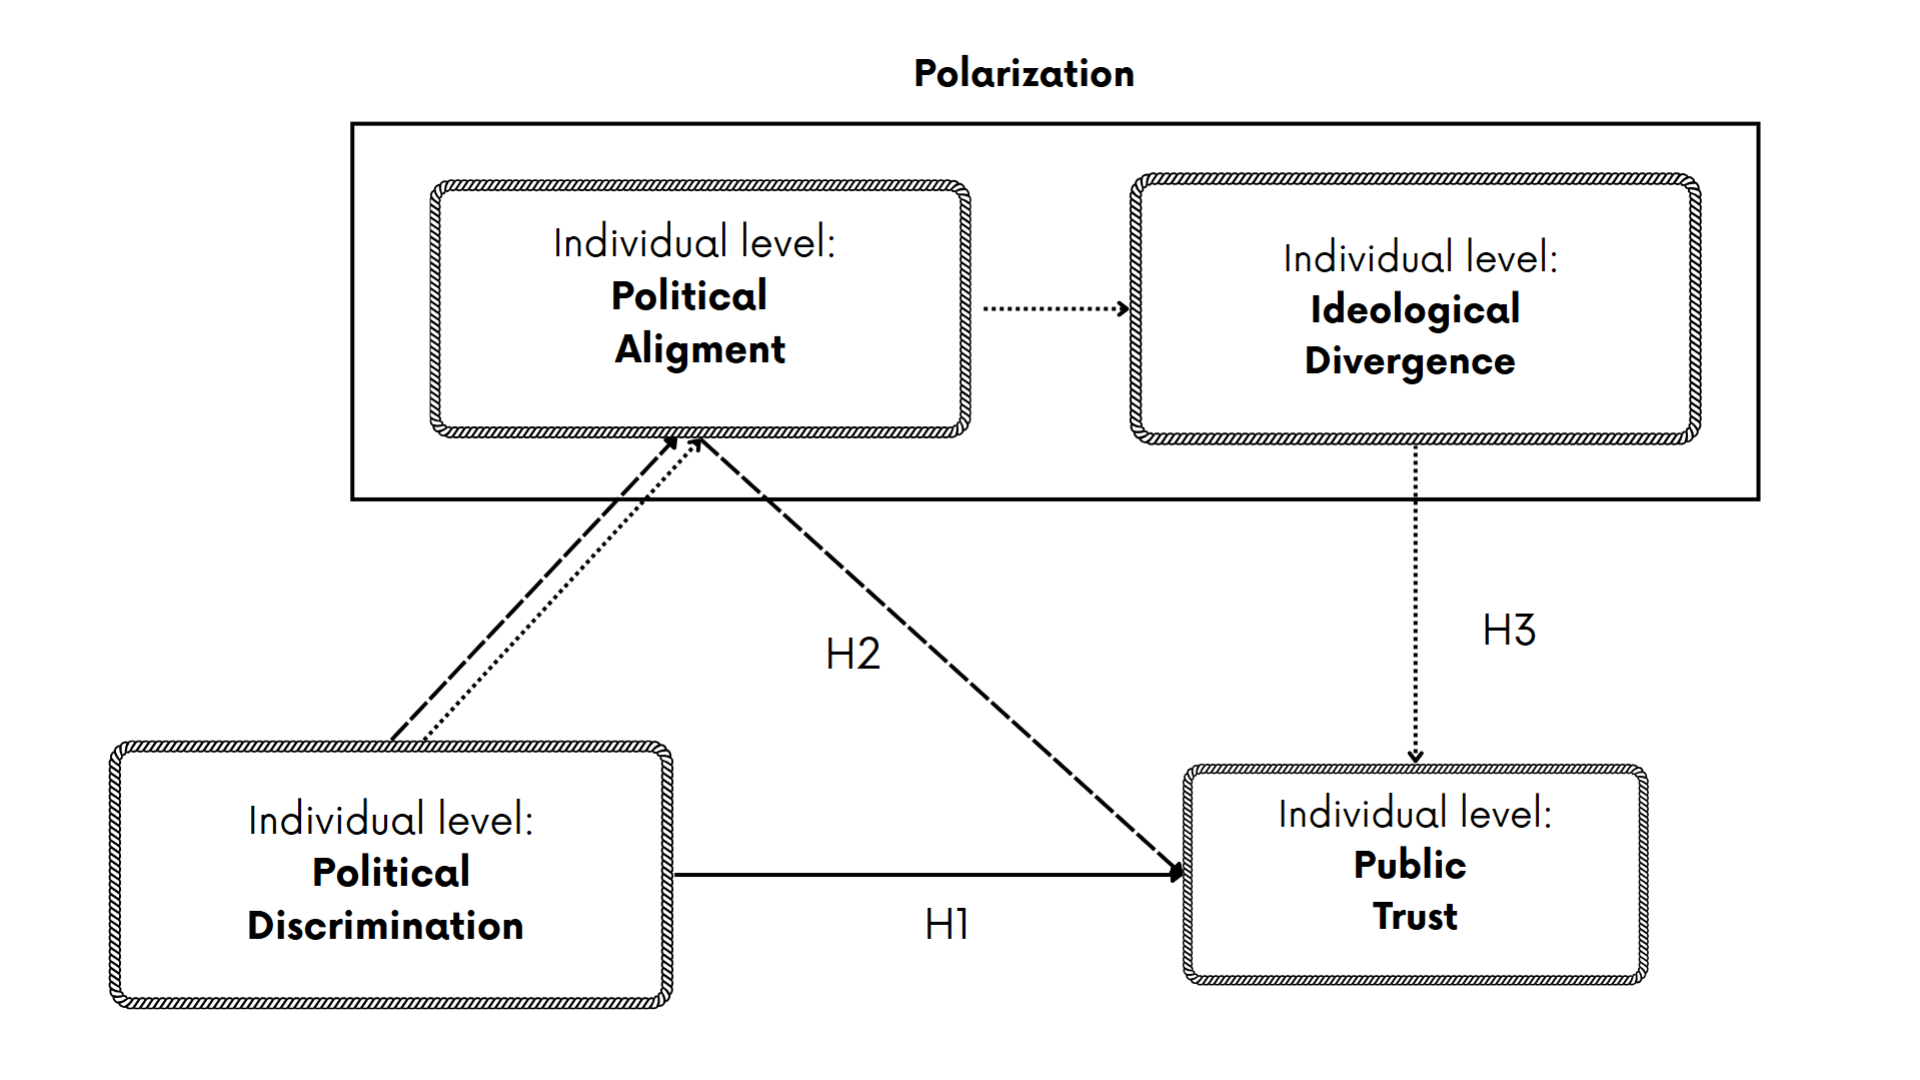
\includegraphics[width=0.9\textwidth]{"viz/theoretical_diagram.png"}
\end{figure}

In polarized environments, this grievance deepens. Political disagreement becomes moral antagonism, and institutions are increasingly interpreted through partisan lenses. Even neutral bodies are recast as political actors, distorting legitimacy and undermining the institutional consensus on which democratic stability relies.

Ultimately, the interaction between political discrimination and polarization does not produce a uniform decline in trust. Instead, it fragments perceptions of legitimacy. Those who feel ideologically marginalized are more likely to view institutions as biased or adversarial, while those who feel politically represented may retain confidence. These mechanisms reinforce one another, compounding democratic disaffection, deepening polarization, and threatening the foundations of pluralistic governance.

\section{Data}

This study uses microdata from general population surveys collected in all 27 European Union Member States as part of the \emph{EUROVOICES} project, conducted by \textcite{the_world_justice_project}.\footnote{The World Justice Project \emph{EUROVOICES} was a data collection effort that aimed to evaluate, analyze, and map out national and regional variations in how people in the EU perceive and experience democratic governance, fundamental rights, justice, safety, corruption, transparency, regulatory enforcement, and the business climate \parencite{the_world_justice_project}.} The dataset provides statistically representative coverage across 110 subnational regions throughout the European Union, offering comprehensive geographic representation of the EU population.

The World Justice Project produced subnational information following the framework of territorial divisions established by the Nomenclature of Territorial Units for Statistics (NUTS) system. In each covered country, one level of this system of nested territorial divisions was selected (NUTS-1 or NUTS-2), resulting in a total of 110 subnational regions. It should be noted that the level of statistical representation varies between countries.

The surveys were administered to respondents in 110 regions of the 27 EU Member States. Data collection employed mixed methodologies, with face-to-face interviews conducted in ten countries and online polling conducted in 17 countries. Survey respondents in each country-region were selected using probability sampling methods designed to ensure representativeness across key sociodemographic criteria, including age, sex, income level, and degree of urbanization (categorized as urban and rural areas). Detailed information on sample sizes for each country, survey methodology employed, data collection periods, and representation levels can be found in Appendix \ref{appendix:a}.

Due to missing values across the variables of interest, the effective analytical sample for this study is smaller than the total sample published by The World Justice Project. Table \ref{table:1} presents descriptive statistics for the key demographic and political variables among survey respondents included in the study \emph{full} sample.

\begin{table}[hbtp]
\centering
\caption{Sample Demographics and Political Preferences}
\label{table:1}
\footnotesize
\vspace{2mm}
\begin{talltblr}[         %% tabularray outer open
label=none,
note{†} = {Classified as ``\emph{constrained}" if respondents mentioned that their income is not enough fo basic necessities or clothing and ``\emph{unconstrained}" otherwise.},
note{‡} = {Individuals had to answer if they were very interested, interested, a little interested, or not at all interested in politics.},
note{§} = {Political alignment was captured using the respondents' vote intention, where they had to pick a political party to vote for if the general elections were happening that weekend.},
remark{Source} = {Eurovoices General Population Poll 2024},
]                     %% tabularray outer close
{                     %% tabularray inner open
colspec={Q[]Q[]Q[]Q[]Q[]Q[]},
hline{4}={1,2,3,4,5,6}{solid, black, 0.1em},
}                     %% tabularray inner close
\toprule
& Unique & Mean & SD & Min & Max \\ \midrule %% TinyTableHeader
Age & 79 & 49.7 & 16.6 & 18.0 & 99.0 \\
Political Ideology & 11 & 5.4 & 2.3 & 0.0 & 10.0 \\
&  & N & \% &  &  \\
Sex & Female & 22,659 & 51.2 &  &  \\
& Male & 21,576 & 48.8 &  &  \\
Area of Residence & Urban & 31,993 & 72.3 &  &  \\
& Rural & 12,242 & 27.7 &  &  \\
Employment & Employed & 24,821 & 56.1 &  &  \\
& Unemployed/Inactive & 19,414 & 43.9 &  &  \\
Citizenship Status & Citizen & 43,224 & 97.7 &  &  \\
& Foreigner & 1,011 & 2.3 &  &  \\
Marital Status & Married & 26,838 & 60.7 &  &  \\
& Not married & 17,397 & 39.3 &  &  \\
Ethnic Group & Ethnic Majority & 26,629 & 60.2 &  &  \\
& Ethnic Minority & 17,606 & 39.8 &  &  \\
Financial Situation\TblrNote{†} & Constrained & 10,103 & 22.8 &  &  \\
& Unconstrained & 34,132 & 77.2 &  &  \\
Education & Higher Education & 14,278 & 32.3 &  &  \\
& No Higher Education & 29,957 & 67.7 &  &  \\
Interest in Politics\TblrNote{‡} & Interested & 21,887 & 49.5 &  &  \\
& Uninterested & 22,348 & 50.5 &  &  \\
Political Alignment\TblrNote{§} & Incumbent Political Party & 7,742 & 17.5 &  &  \\
& Non-Incumbent Political Party & 36,493 & 82.5 &  &  \\
Political D/H & D/H Experience & 7,002 & 15.8 &  &  \\
& No D/H Experience & 37,233 & 84.2 &  &  \\
\bottomrule
\end{talltblr}
\end{table}


The \emph{EUROVOICES} survey includes a comprehensive discrimination module that measures 11 different grounds for discrimination: sex, age, disability, ethnicity, migration background, socioeconomic status, religion, and political opinion. Participants indicated whether they experienced discrimination or harassment (D/H) based on any of these characteristics during the 12 months before the survey, and identified where such incidents took place. Since each discrimination ground was assessed independently, individual respondents could report multiple types of discriminatory experiences within the year prior to survey administration.

The survey also includes a comprehensive Trust module asking respondents to rate their trust levels in various public institutions as ``a lot", ``some", ``a little", or ``no trust". These institutions include local and national government officials, police officers, prosecutors, public defense attorneys, judges, magistrates, political parties, and Parliament members. We recoded these responses into binary indicators, where ``a lot" and ``some trust" equal 1, and ``a little" and ``no trust" equal 0. To construct a comprehensive measure of political trust, we created a Trust in Political Institutions Index through Logistic Principal Component Analysis \parencite{landgraf_dimensionality_2020}, which aggregates individual trust responses across all measured institutions.

Finally, as displayed in Table \ref{table:1}, the survey not only collects important demographic data but it also asks respondents key political traits such as their interest in politics, vote intention, and it also asks people to rate their political ideology from 0 to 10, where 0 is associated with a further left ideology and 10 is associated with a further right ideology.

\section{Discrimination Experiences in the European Union}

Data from the World Justice Project \emph{EUROVOICES} household survey reveals that discrimination represents a significant challenge throughout the European Union. In most EU regions, over 25\% of respondents reported experiencing some form of discrimination within the previous year. Table \ref{table:2} displays the prevalence of self-reported discrimination across EU Member States, categorized by the grounds for discrimination.

Political discrimination represents the most frequently reported form of discrimination in 13 of the 27 members, surpassing discrimination based on sex, ethnicity, or migration status. The highest rates are observed in Hungary (34.5\%), Czechia (28.7\%), Slovakia (26.5\%), Austria (25.3\%), and Germany (24.4\%), while Portugal (2.6\%) and Bulgaria (1.5\%) show considerably lower prevalence. Across the EU, an average of 14.7\% of respondents have encountered political discrimination.

One reason why political grounds for discrimination display such high incidence rates across most countries in our sample is that, unlike other grounds such as sex, ethnicity, or religion, political discrimination affects all demographic groups in our sample. While political opinion may not be the predominant form of discrimination experienced by specific minority or marginalized groups, they become the most common ground when considering the entire population. This pattern reflects the universal nature of political discrimination—it can target individuals regardless of their demographic characteristics.

These findings indicate that political discrimination constitutes a prominent and pervasive issue across numerous European contexts. Notably, this form of discrimination has become more prevalent than traditionally recognized categories of discrimination in a substantial number of countries, suggesting an evolution in the nature of exclusionary experiences faced by individuals.

\begin{table}
\centering
\begin{talltblr}[         %% tabularray outer open
entry=none,label=none,
note{}={*Note*: Table displays the percentage of respondents in each country that answered to have had experienced discrimination
  or harrasment for each of the grounds presented to them by the survey.},
]                     %% tabularray outer close
{                     %% tabularray inner open
colspec={Q[]Q[]Q[]Q[]Q[]Q[]Q[]Q[]Q[]},
column{3,4,5,6,7,8,9}={}{halign=c,},
column{1,2}={}{halign=l,},
}                     %% tabularray inner close
\toprule
& Country & Political Opinion & Sex & Gender & Ethnicity & Migration Status & Social Status & Religion \\ \midrule %% TinyTableHeader
& Austria & \num{25.3} & \num{13.0} & \num{9.5} & \num{13.1} & \num{12.6} & \num{17.8} & \num{11.6} \\
& Belgium & \num{13.2} & \num{15.0} & \num{8.5} & \num{13.0} & \num{9.2} & \num{18.1} & \num{10.7} \\
& Bulgaria & \num{1.5} & \num{1.8} & \num{0.7} & \num{2.1} & \num{0.6} & \num{3.1} & \num{1.1} \\
& Croatia & \num{11.8} & \num{8.2} & \num{2.6} & \num{5.0} & \num{3.1} & \num{11.2} & \num{8.3} \\
& Cyprus & \num{11.0} & \num{13.3} & \num{6.1} & \num{6.4} & \num{5.5} & \num{12.3} & \num{6.7} \\
& Czechia & \num{28.7} & \num{13.0} & \num{10.0} & \num{13.9} & \num{16.6} & \num{18.5} & \num{5.4} \\
& Denmark & \num{11.5} & \num{13.0} & \num{7.5} & \num{10.8} & \num{9.9} & \num{14.7} & \num{10.1} \\
& Estonia & \num{15.5} & \num{9.5} & \num{3.4} & \num{6.7} & \num{2.2} & \num{10.1} & \num{2.8} \\
& Finland & \num{13.7} & \num{11.4} & \num{4.6} & \num{4.4} & \num{2.8} & \num{15.9} & \num{5.0} \\
& France & \num{10.4} & \num{11.6} & \num{4.6} & \num{7.7} & \num{4.4} & \num{12.2} & \num{6.7} \\
& Germany & \num{24.4} & \num{11.9} & \num{8.0} & \num{11.1} & \num{10.0} & \num{16.0} & \num{9.5} \\
& Greece & \num{5.2} & \num{3.6} & \num{0.8} & \num{1.5} & \num{1.4} & \num{2.8} & \num{1.0} \\
& Hungary & \num{34.5} & \num{15.9} & \num{16.5} & \num{22.4} & \num{16.5} & \num{27.8} & \num{14.3} \\
& Ireland & \num{12.7} & \num{15.8} & \num{7.1} & \num{9.1} & \num{8.7} & \num{14.8} & \num{9.6} \\
& Italy & \num{13.7} & \num{13.7} & \num{7.8} & \num{8.1} & \num{6.3} & \num{13.9} & \num{8.2} \\
& Latvia & \num{6.0} & \num{2.5} & \num{0.5} & \num{7.5} & \num{1.9} & \num{5.5} & \num{1.9} \\
& Lithuania & \num{5.3} & \num{2.2} & \num{0.1} & \num{2.9} & \num{0.5} & \num{4.9} & \num{1.0} \\
& Malta & \num{13.0} & \num{6.8} & \num{1.6} & \num{4.4} & \num{3.4} & \num{4.4} & \num{4.0} \\
& Netherlands & \num{15.2} & \num{14.0} & \num{9.4} & \num{12.5} & \num{11.2} & \num{15.2} & \num{10.6} \\
& Poland & \num{6.7} & \num{3.0} & \num{1.0} & \num{1.3} & \num{1.0} & \num{3.4} & \num{2.4} \\
& Portugal & \num{2.6} & \num{3.5} & \num{2.6} & \num{4.1} & \num{2.8} & \num{4.1} & \num{3.5} \\
& Romania & \num{4.7} & \num{3.6} & \num{1.8} & \num{3.7} & \num{1.7} & \num{5.3} & \num{2.7} \\
& Slovakia & \num{26.5} & \num{14.1} & \num{10.7} & \num{12.3} & \num{10.1} & \num{18.5} & \num{11.1} \\
& Slovenia & \num{18.1} & \num{10.1} & \num{5.3} & \num{9.2} & \num{7.1} & \num{17.0} & \num{9.0} \\
& Spain & \num{19.8} & \num{14.6} & \num{7.5} & \num{9.4} & \num{8.4} & \num{15.2} & \num{8.3} \\
& Sweden & \num{12.1} & \num{15.3} & \num{5.7} & \num{10.8} & \num{7.2} & \num{13.4} & \num{7.3} \\
\bottomrule
\end{talltblr}
\end{table}


\section{Methodology}

The main objective of this study is to examine whether experiencing discrimination or harassment due to political opinions has a causal effect on trust in political institutions (H1). However, a fundamental challenge in causal inference is that assessing the causal effect of these experiences would require observing both potential outcomes in the same individual—those who experienced a D/H event and those who did not. Since we never observe both potential outcomes for any individual, we must infer the effects of political discrimination and harassment by comparing average trust levels between those who experienced such events and those who did not.

The problem is that people who experience political discrimination or harassment might be systematically different from those who do not. For example, individuals who experience such events might be more interested in and informed about politics, or display higher levels of civic participation. If these systematic differences correlate with institutional trust levels, then a naïve comparison between the two groups would be misleading. This is known as the selection problem \parencite{angrist_mostly_2009}.

Researchers typically turn to randomized controlled experiments—the gold standard for causal inference—to address such questions. However, the nature of our research question makes it both practically difficult and ethically problematic to randomly expose individuals to discrimination or harassment based on their political views. As a result, we adopt quasi-experimental designs to examine the causal effects of political discrimination and harassment on institutional trust.

For this study, we implement the matching methodology suggested by \textcite{ho_matching_2007} to preprocess our observational data. Our goal is to balance the distribution of covariates between our treatment group (people who experienced D/H events) and control group (people who have not), thereby replicating the randomization achieved in an experimental study \parencite{stuart_matching_2010}.

While regression methods can also address confounding from measured covariates, using regression on matched samples reduces the dependence of our treatment effect estimates on correct model specification. This approach provides more robust causal inferences by making the groups more comparable before applying statistical models.

Importantly, we use matching as a preprocessing method to improve balance between groups, rather than as an imputation method for estimating missing outcomes, as described by \textcite{abadie_large_2006, abadie_matching_2016}.

We performed nearest neighbor matching\footnote{The matching estimation was performed using the MatchIT R package \parencite{ho_matchit_2011}.} based on the propensity score, defined as the probability of experiencing a D/H event conditional on a set of observed covariates \parencite{rubin_matching_1973, rosenbaum_central_1983}. We estimate this probability using a logistic regression. Each unit from the treatment group is matched with the control group unit that has the closest propensity score (1:1 matching without replacement)\footnote{Matching with replacement means that each control unit can be reused to be matched with any number of treated units if that individual is the closest neighbor to multiple treatment units. Matching without replacement means that each control unit can only be matched with one single treated unit.}. We also establish a region of common support\footnote{The common support region refers to the range of covariate values (or propensity scores) where both treated and control units have sufficient representation.} and discard units that fall outside this region.\footnote{All treatment units fell within the common support region, resulting only in exclusion of individuals from the control group, i.e., people who did not experience political discrimination or harassment.}

The propensity score is estimated using two sets of covariates: demographic variables (geographic region,\footnote{Equivalent to one of the 110 NUTS regions in the study.} sex, age, area of residence, financial situation, education level, employment status, marital status, citizenship status, and ethnic group) and political variables (interest level in politics, political ideology, and political alignment). All covariates and their possible values are listed in Table \ref{table:1}.

Once we have a fully matched study sample, we estimate the effect of having experienced a D/H event on the levels of trust in political institutions through the following specification:

\begin{equation}
\label{eq:1}
log(Y_{ic}) = \alpha + \tau X_{ic} + \mathbf{Z}_{ic}'\mathbf{\beta} + \gamma_c + \varepsilon_{ic}
\end{equation}

Where:
\begin{itemize}
  \item \( Y_{ic} \): political trust for individual \( i \) in region \( c \)
  \item \( X_{ic} \): D/H event (1 = treated, 0 = control)
  \item \( \tau \): treatment effect (ATT)
  \item \( \mathbf{Z}_{ic} \): vector of covariates
  \item \( \mathbf{\beta} \): coefficient vector for covariates
  \item \( \gamma_c \): region fixed effects
  \item \( \varepsilon_{ic} \): error term
\end{itemize}

This specification is estimated using fixed effects OLS regression\footnote{The estimation of the fixed effects was performed using the fixest R package \parencite{berge_efficient_2018}.}. The value of \( \tau \) can be interpreted as the Average Treatment Effect on the Treated (ATT)\footnote{The Average Treatment Effect (ATE) and the Average Treatment Effect on the Treated (ATT) are two foundational metrics in causal inference. ATE represents the average effect of a treatment across the entire population, whereas ATT focuses only on the average effect among individuals who actually received the treatment.} provided that the conditional ignorability (unconfoundedness) assumption holds \parencite{abadie_econometric_2018, greifer_matching_2021}.

The unconfoundedness assumption requires that treatment assignment be independent of potential outcomes conditional on the set of observed covariates included. However, even when matching achieves balance in observed covariates, unobserved confounders remain a threat to causal identification. Unobserved variables that relate to both experiencing D/H events and trust in political institutions would violate the unconfoundedness assumption and bias our treatment effect estimates. Since conditional ignorability cannot be directly tested, the literature suggests performing sensitivity analyses to assess the plausibility of this assumption and determine how sensitive our estimated effects are to violations of unconfoundedness \parencite{stuart_matching_2010}.

We use the framework proposed by \textcite{cinelli_making_2020} to assess how fragile are our main results to the possibility of unobserved confounding. This framework allows us to estimate the minimum strength of an unobserved confounder that would be required to nullify our estimated treatment effect. We also assess the robustness of our results to violations of the unconfoundedness assumption by estimating the treatment effect under different levels of unobserved confounding.

We use two measures to test the sensitivity of our results: the robustness value, indicating the minimum confounding strength needed to alter our conclusions, and the partial R2 of the treatment, showing how strongly confounders must be associated with the treatment to completely override our results \parencite{cinelli_making_2020}.\footnote{The practical implementation of the sensitivity analysis was performed using the sensemakr R package \parencite{cinelli_sensemakr_2024}.}

As outlined in our study hypotheses (H2 and H3), we also examine whether the effect of experiencing political discrimination or harassment varies according to an individual’s political alignment and ideological divergence. To test these hypotheses, we introduce interaction terms that allow us to assess whether the relationship between experiences of political discrimination and trust in political institutions is moderated by a third factor.

First, we include an interaction term between the D/H event variable and political alignment with the incumbent party. Political alignment is measured using a vote intention question included in the survey, which asked respondents who they would vote for if a general election were held in their country that weekend. Respondents who selected the incumbent party are categorized as politically aligned, while all others are considered unaligned (see Equation \ref{eq:4}).

Second, we introduce an additional layer of analysis by interacting the D/H event variable with a new measure of ideological divergence. To construct this variable, we follow a similar approach to \textcite{torcal_ideological_2022}, who capture ideological extremism as the distance between an individual’s ideological self-placement and the societal center—an operationalization of ideological polarization.\footnote{\textcite{torcal_ideological_2022} use this approach to measure ideological extremism, which they conceptualize as a manifestation of broader ideological polarization.}

Respondents were asked to place themselves on a scale from 0 to 10, where 0 represents a further left ideology and 10represents a further right ideology. We then calculate ideological divergence as the squared difference between each respondent's self-placement and the mean ideological position within their respective subnational region (see Equation \ref{eq:4}).

\begin{equation}
  \label{eq:4}
  log(Y_{ic}) = \alpha + \tau X_{ic} + \delta D_{ic} + \phi X_{ic}D_{ic} + \mathbf{Z}_{ic}'\mathbf{\beta} + \gamma_c + \varepsilon_{ic}
  \end{equation}
  
  Where:
  \begin{itemize}
    \item \( Y_{ic} \): political trust for individual \( i \) in region \( c \)
    \item \( X_{ic} \): D/H event (1 = treated, 0 = control)
    \item \( D_{ic} \): pathway (high ideological divergence or political aligned) for individual \( i \) in region \( c \)
    \item \( \tau \): treatment effect (ATT)
    \item \( \delta \): pathway unilateral effect on Trust in Political Institutions Index
    \item \( \phi \): interaction effect between D/H event and political alignment with the incumbent party
    \item \( \mathbf{Z}_{ic} \): vector of covariates
    \item \( \mathbf{\beta} \): coefficient vector for covariates
    \item \( \gamma_c \): region fixed effects
    \item \( \varepsilon_{ic} \): error term
  \end{itemize}

\section{Results}

When we compare trust levels in political institutions between people who have experienced discrimination or harassment (D/H) due to their political opinions and those who have not, we observe that the former group typically achieves lower average scores, as shown in Figure \ref{fig:1}. This figure reveals a strong negative correlation between experiencing D/H events and current levels of institutional trust. However, this relationship cannot be claimed to be causal. As explained previously, people who initially have lower trust in institutions might display higher levels of political participation or activism and, therefore, be more prone to experiencing discrimination.

\begin{figure}[htbp]
\centering
\caption{Trust in Political Institutions by Political D/H Experience}
\label{fig:1}
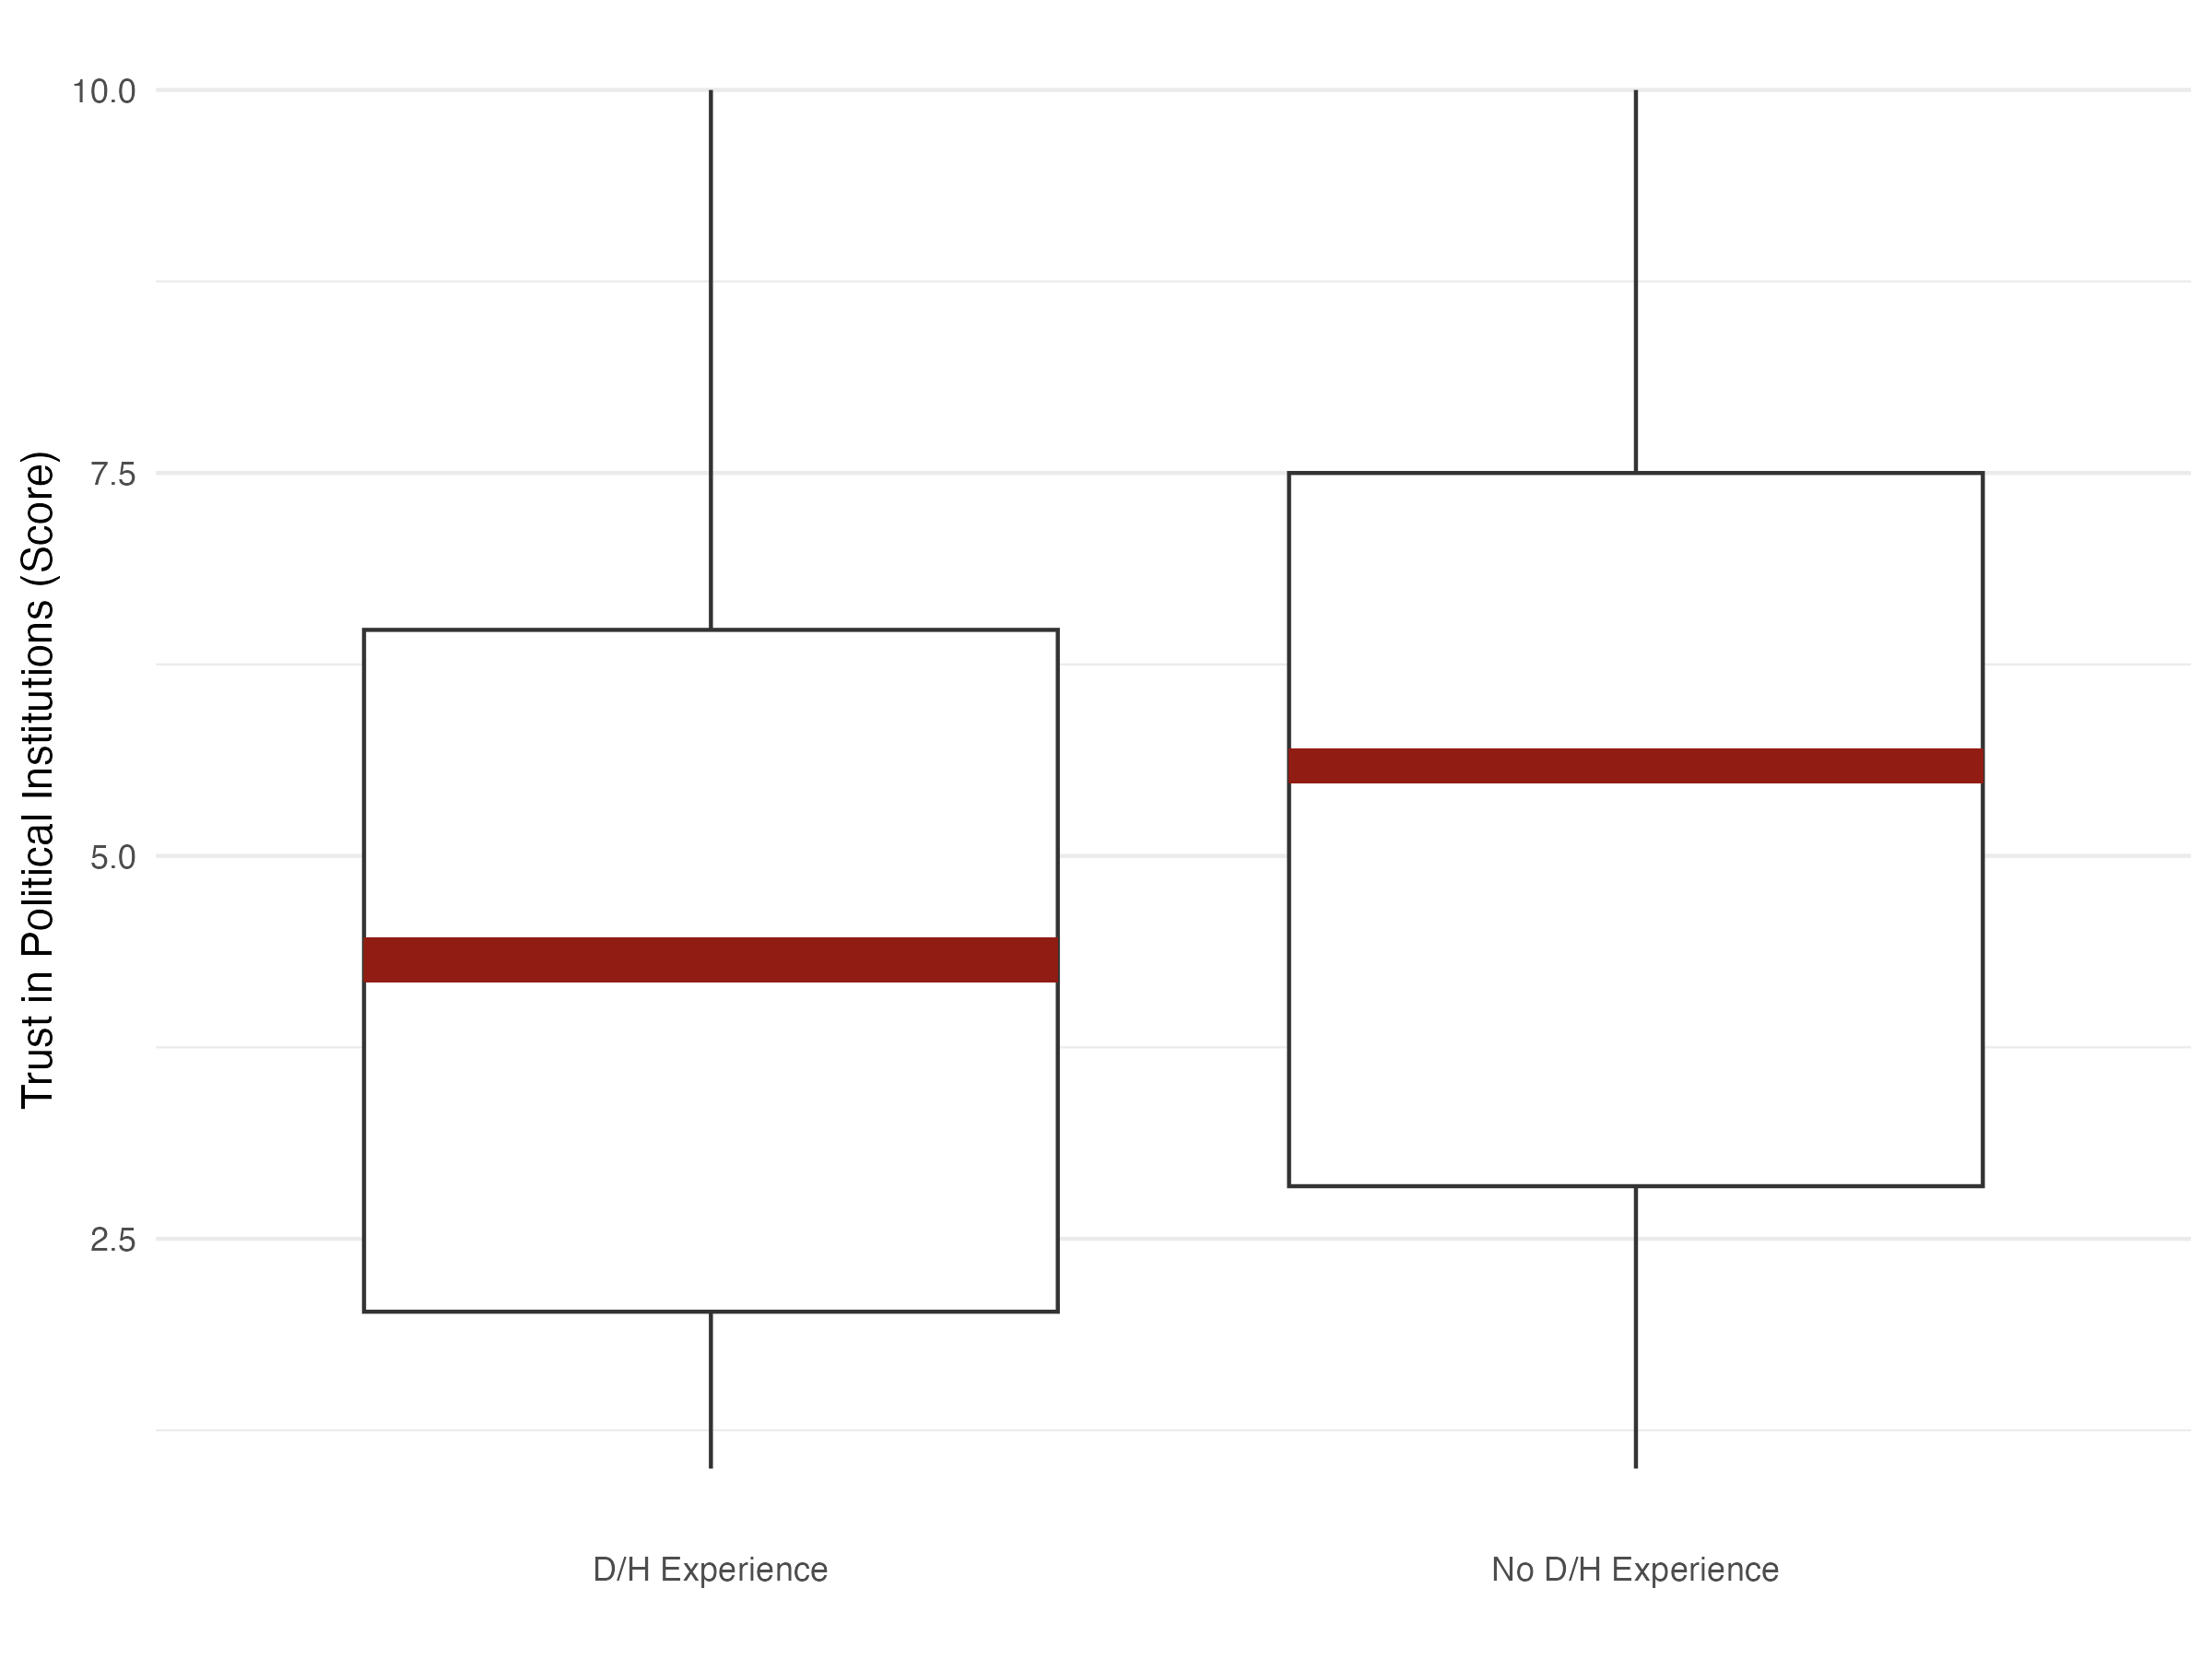
\includegraphics[width=0.9\textwidth]{"viz/fig_trust_comparison_naive.png"}

\medskip
\justifying\footnotesize 
\textit{Note:} The figure shows the distribution of Trust in Political Institutions Index scores for individuals who experienced political discrimination or harassment (D/H) versus those who did not. Index scores are derived from Logistic PCA of trust responses across nine institutional categories: local authorities, national authorities, police, prosecutors, public defense attorneys, judges, magistrates, political parties, and Parliament members. Red areas show 95\% confidence intervals of median scores. Scores were re-scaled to fit a scale between 1-10.

\textit{Source:} Eurovoices General Population Poll 2024
\end{figure}

We attempt to isolate a causal effect by matching people who have experienced a D/H event with people who have similar demographic characteristics and political traits but have not experienced such events. This approach allows us to approximate the counterfactual outcomes that we cannot directly observe in our data. To evaluate how this matching affects our analysis, we begin by assessing the initial balance in characteristics between people who have experienced D/H events and those who have not.

\subsection{Assessing balance between groups}

Appendix \ref{appendix:b} shows balance statistics for the whole sample prior to matching. As we can observe, several covariates display standardized mean differences above the thresholds suggested by the literature—0.1 or, more conservatively, 0.05. Of particular note are the high values for average civic participation, interest in politics, and political alignment with the incumbent party, suggesting that the political profiles of people who have suffered D/H due to their political opinions and those who have not are systematically different. Similarly, age and ethnic composition differ significantly between both groups on average, indicating that the demographic composition of the groups is also systematically different. These insights are validated by the variance ratios and empirical cumulative distribution functions (eCDFs).\footnote{The Std. Mean Diff. is the difference in group means standardized to a single scale for all covariates. The literature suggests values below 0.1—or more conservatively, below 0.05—as indicators of good balance \parencite{ali_propensity_2014, stuart_prognostic_2013}. The Var. Ratio compares the variance of a covariate between the treatment and control groups. Ratios close to 1 indicate good balance \parencite{austin_balance_2009}. Empirical Cumulative Distribution Function Statistics (eCDF) assess balance beyond the mean by comparing the full distribution of each covariate across groups \parencite{mccaffrey_propensity_2004}. Values close to zero indicate good balance.}

The imbalances found between both groups suggest that estimates calculated using the full study sample would carry significant bias due to systematic differences in demographic and political characteristics. Therefore, a matching procedure to preprocess the data is a valid approach to reduce these biases.

After performing the matching procedure, we reassess the balance of covariates between the treatment and control groups. The results are presented in Table \ref{table:3}. As we can see, the matching procedure has significantly improved the balance of covariates between both groups. The standardized mean differences for all covariates are now below 0.05, indicating that the treatment and control groups are now comparable in terms of their demographic and political characteristics. This is further supported by the variance ratios, which are now close to 1 for all covariates, and the empirical cumulative distribution function (eCDF) statistics, which are also close to zero for all covariates. Appendix \ref{appendix:c} provides a love plot that visually summarizes the balance of covariates before and after matching.

\begin{table}[hbtp]
\centering
\caption{Post-Matching Covariate Balance Assessment}
\label{table:3}
\footnotesize
\vspace{2mm}
\begin{talltblr}[
label=none,
remark{Note} = {The Std. Mean Diff. is the difference in group means standardized to a single scale for all covariates. The literature suggests values below 0.1—or more conservatively, below 0.05—as indicators of good balance (Ali et al., 2011; Stuart et al., 2013). The Var. Ratio compares the variance of a covariate between the treatment and control groups. Ratios close to 1 indicate good balance (Austin, 2009). Empirical Cumulative Distribution Function Statistics (eCDF) assess balance beyond the mean by comparing the full distribution of each covariate across groups (McCaffrey et al., 2004). Values close to zero indicate good balance.},
remark{Source} = {Eurovoices General Population Poll 2024},
]
{                     
colspec={Q[l]Q[c]Q[c]Q[c]Q[c]Q[c]Q[c]},
% hline{4}={1,2,3,4,5,6}{solid, black, 0.1em},
}                   
\toprule
  & \makecell{Mean\\D/H Exp.} & \makecell{Mean\\No D/H Exp.} & \makecell{Std. Mean\\Diff.} & \makecell{Var.\\Ratio} & \makecell{eCDF\\Mean} & \makecell{eCDF\\Max} \\ 
\midrule
Distance & 0.270 & 0.265 & 0.031 & 1.122 & 0.001 & 0.027\\
Female & 0.468 & 0.461 & 0.014 & - & 0.007 & 0.007\\
Age & 46.268 & 46.255 & 0.001 & 1.000 & 0.004 & 0.013\\
Rural & 0.244 & 0.243 & 0.002 & - & 0.001 & 0.001\\
\makecell[l]{Constrained Fin.\\Situation} & 0.281 & 0.269 & 0.027 & - & 0.012 & 0.012\\
Higher Education & 0.352 & 0.358 & -0.013 & - & 0.006 & 0.006\\
Employed & 0.579 & 0.584 & -0.010 & - & 0.005 & 0.005\\
Married & 0.570 & 0.580 & -0.019 & - & 0.010 & 0.010\\
Foreigner & 0.025 & 0.025 & 0.002 & - & 0.000 & 0.000\\
Ethnic Minority & 0.513 & 0.512 & 0.003 & - & 0.001 & 0.001\\
Interest in Politics & 0.663 & 0.658 & 0.011 & - & 0.005 & 0.005\\
Political Ideology & 5.504 & 5.485 & 0.008 & 1.153 & 0.017 & 0.033\\
\makecell[l]{Political Al.\\with Incumbent} & 0.117 & 0.121 & -0.012 & - & 0.004 & 0.004\\
\makecell[l]{Civic Participation\\Score} & -2.499 & -2.570 & 0.015 & 1.015 & 0.010 & 0.024\\
\midrule
\textit{Sample sizes:} & \textit{Control} & \textit{Treated} & & & & \\
All & 37,233 & 7,002 & & & & \\
Matched & 7,002 & 7,002 & & & & \\
Unmatched & 30,184 & 0 & & & & \\
Discarded & 47 & 0 & & & & \\
\bottomrule
\end{talltblr}
\end{table}


As a result of the matching procedure, our sample size was reduced from 44,235 individuals to 14,004 individuals. The final matched sample consists of 7,002 individuals who experienced D/H events and 7,002 individuals who did not. This reduction in sample size is a common outcome of matching procedures, as some individuals may not have suitable matches in the control group or may fall outside the common support region. This is the study sample we use to estimate the causal effect of political discrimination and harassment on trust in political institutions.

\subsection{The effect of political discrimination and harassment on trust in political institutions}

To estimate the effect of political discrimination and harrasment on trust in political institutions, we estimate four different specifications of Equation \ref{eq:1}. The first specification includes only the treatment variable (experiencing a D/H event) and region fixed effects. The second specification adds demographic covariates, while the third specification adds both demographic and political covariates. The fourth specification replicates the third one, but it fits the model using the full unmatched sample. The results of these estimations are presented in Table \ref{table:4}.

\begin{table}
\centering
\begin{tblr}[         %% tabularray outer open
]                     %% tabularray outer close
{                     %% tabularray inner open
colspec={Q[]Q[]Q[]Q[]Q[]},
column{2,3,4,5}={}{halign=c,},
column{1}={}{halign=l,},
hline{3}={1,2,3,4,5}{solid, black, 0.05em},
}                     %% tabularray inner close
\toprule
& (I) & (II) & (III) & (IV) \\ \midrule %% TinyTableHeader
D/H Experience & \num{-0.194}*** & \num{-0.191}*** & \num{-0.189}*** & \num{-0.159}*** \\
Num.Obs. & \num{14004} & \num{14004} & \num{14004} & \num{44235} \\
Adj. R.sq. & 0.074 & 0.090 & 0.110 & 0.101 \\
Adj. Within R.sq. & 0.022 & 0.039 & 0.060 & 0.046 \\
Region FE & X & X & X & X \\
Dem. Cov. &  & X & X & X \\
Pol. Cov. &  &  & X & X \\
Sample & Matched & Matched & Matched & Full \\
\bottomrule
\end{tblr}
\end{table}


As we can observe, the coefficient for the D/H event variable is negative and statistically significant in all specifications. This indicates that experiencing political discrimination or harassment has a negative effect on trust in political institutions. Furthermore, the magnitude of this effect is consistent across specifications, ranging from -0.159 to -0.194, depending on the model. This means that individuals who have experienced political discrimination or harassment tend to have between 16\% and 19\% lower levels of trust in political institutions compared to those who have not experienced such events. This effect is large in the context of public opinion data and suggests a meaningful deterioration in institutional trust linked to experiences of political unfairness or targeting.

Interestingly, the magnitude of the coefficient is slightly smaller when using the full unmatched sample, which suggests that the bias introduced by using the full sample tends to underestimate the absolute effect of political discrimination and harassment on trust in political institutions.

Using a matched sample has allowed us to improve the precision of our estimates. However, achieving a balance in covariates using a matching procedure suggests that the treatment and control groups are comparable in ways that are more aligned with the assumptions necessary for causal inference \parencite{branson_randomization_2021}. However, balance represents a necessary but not sufficient condition for causality, as unobserved confounders may still bias our estimates. Therefore, we perform a sensitivity analysis to assess the robustness of our results to potential violations of the unconfoundedness assumption.

\subsection{Sensitivity analysis}

We assess the robustness of our results to violations of the unconfoundedness assumption using the sensitivity analysis framework of \textcite{cinelli_making_2020}. This method estimates the minimum strength of unobserved confounding needed to eliminate our treatment effect and evaluates how results vary under different confounding scenarios. Table \ref{table:5} presents these sensitivity analysis results.

According to our results, the robustness value ($RV_{q = 1}$) is 13.8\%, which means that an unobserved confounder—orthogonal to the current set of covariates—would need to explain at least 13.8\% of the variance in experiencing political discrimination or harassment (D/H) to nullify our estimated treatment effect.

Similarly, the robustness value for testing the null hypothesis that the treatment effect is zero ($RV_{q = 1, \alpha = 0.05}$) is 12.4\%. This means that an unobserved confounder—orthogonal to the current set of covariates—would need to explain at least 12.4\% of the variance in experiencing D/H events to make our treatment effect statistically insignificant at the 5\% level.

Finally, the partial $R^2$ of the treatment ($R^2_{Y\sim D| {\bf X}, D}$) is 3.5\%, which indicates that an unobserved confounder would need to explain at least 3.5\% of the variance in trust in political institutions to nullify our estimated treatment effect.

These levels are relatively high. However, without accurate domain knowledge, it is very difficult to assess how strong the unobserved factors not captured in our data might be. To provide context, we benchmark these results against political alignment with the incumbent party—a covariate strongly related to institutional trust. Political alignment serves as a reasonable upper bound since few omitted variables would likely have stronger associations with institutional trust and D/H experiences than alignment with the governing party.

Table \ref{table:5} shows the benchmarking results for political alignment with the incumbent party (\emph{incpp}). According to the analysis, political alignment explains only 1.8\% of the variance in trust in political institutions, which is significantly lower than the estimated partial $R^2$ and both RV values. Therefore, we can conclude that our results are robust to the possibility of unobserved confounding.

\begin{table}[hbtp]
\centering
\caption{Sensitivity Analysis: Main Results}
\label{table:5}
\footnotesize
\vspace{2mm}
\begin{talltblr}[
label=none,
% remark{Note} = {Table shows the results of regressing having experienced political discrimination or harrasment (D/H) on the level of trust in political institutions, measured as an index score. Model (I) includes only the treatment variable (D/H event) and region fixed effects. Model (II) adds demographic covariates, while model (III) and (IV) adds both demographic and political covariates. Model (IV) uses the full unmatched sample to fit the regression. *, **, and *** represent statistical significance at p < 0.05, p < 0.01, and p < 0.001, respectively. Standard Errors are clustered at the regional level and paired-units weights were used for regressions using the matched sample.},
remark{Source} = {Eurovoices General Population Poll 2024},
]
{                     
colspec={Q[l]Q[c]Q[c]Q[c]Q[c]Q[c]Q[c]},
colsep=4pt
}
\toprule
\textbf{Treatment:} & \textbf{Est.} & \textbf{S.E.} & \textbf{t-value} & $R^2_{Y \sim D |{\bf X}}$ & $RV_{q = 1}$ & $RV_{q = 1, \alpha = 0.05}$  \\ 
\midrule 
\textit{D/H Experience} & -0.209 & 0.012 & -17.523 & 2.2\% & 13.8\% & 12.4\% \\ 
\bottomrule 
df = 13,880 & & \SetCell[r=1,c=5]{r} { \small \textit{Bound (2x incpp)}: $R^2_{Y\sim Z| {\bf X}, D}$ = 1.8\%, $R^2_{D\sim Z| {\bf X} }$ = 0\%} \\
\end{talltblr}
\end{table}


Our analysis further shows that results remain valid even with an omitted confounder 15 times stronger than political alignment (see Appendix \ref{appendix:d}). Moreover, the treatment effect magnitude remains stable even under this extreme confounding scenario. This reinforces our conclusion that the results are robust to unobserved confounding, at least within the bounds established by our political alignment benchmark.

% \subsection{Polarization as a transmission channel}

% As mentioned earlier, we hypothesize that political polarization serves as a transmission channel through which political discrimination and harassment affect trust in political institutions. To test this hypothesis, we conduct a mediation analysis using the framework developed by Imai et al. (2011) and Imai and Yamamoto (2013). This analysis aims to determine how much of the total effect of D/H experiences on institutional trust operates through political polarization. The framework is based in the estimation of the system presented by equations \ref{eq:2} and \ref{eq:3} along with a bootstrapping procedure to test the mediation channel.

% Table \ref{table:6} presents three key estimates: the total effect, the average causal mediation effect (ACME), and the average direct effect (ADE). As we can observe, experiencing political discrimination or harassment leads to a large and highly significant drop in institutional trust: the Total Effect of –0.863 (on a 0–10 scale) tells us that, on average, those who report discrimination score 0.863 points lower in trust than those who do not. This effect is equivalent to the 18.9\% decrease presented in Table \ref{table:4}, column (III).

% To better understand the mechanisms behind this decline in trust, the analysis separates the effect into two components: the part that operates indirectly through increased political dissonance (the Average Causal Mediation Effect, or ACME), and the part that operates directly, independently of dissonance (the Average Direct Effect, or ADE).

% The estimated ACME is –0.0063, meaning that only about 0.006 points of the decline in trust can be attributed to a pathway where discrimination increases political dissonance, which in turn lowers trust. By contrast, the ADE is –0.857, nearly identical to the total effect, which shows that the vast majority of the impact of discrimination on trust occurs directly, without being mediated by political dissonance.

% In other words, less than 1\% of the total effect of political discrimination on institutional trust can be explained by changes in political dissonance. Although this indirect effect is statistically significant, it is substantively negligible. This implies that political dissonance does act as a mechanism, but it plays only a very minor role. Most of the loss in trust stems from other pathways—perhaps emotional responses like anger or fear, cognitive assessments of systemic injustice, or broader alienation from the political system that are not captured by the dissonance variable.

% \begin{table}[hbtp]
\centering
\caption{Mediation Analysis Results}
\label{table:6}
\footnotesize
\vspace{2mm}
\begin{talltblr}[
label=none,
remark{Note} = {Table shows the results of the mediation analysis. The ACME (Average Causal Mediation Effect) measures the indirect effect of having experienced D/H events on trust in political institutions through our measure of affective polarization (\emph{mediator}). The ADE (Average Direct Effect) measures the direct effect on the outcome. The Total Effect is the sum of the ACME and ADE. The Prop. Mediated is the proportion of the total effect that is mediated through the mediator. *, **, and *** represent statistical significance at $p < 0.05$, $p < 0.01$, and $p < 0.001$, respectively. Estimates shown in the table tested using a bootstrapping approach with 10,000 replications.},
remark{Source} = {Eurovoices General Population Poll 2024},
]
{                     
colspec={Q[l]Q[c]Q[c]Q[c]Q[c]},
}                   
\toprule
& Estimate & 95\% CI Lower & 95\% CI Upper & p-value\\
\midrule
ACME & -0.006 & -0.013 & -0.001 & \num{0.02}*\\
ADE & -0.857 & -0.945 & -0.770 & \num{0.00}***\\
Total Effect & -0.863 & -0.951 & -0.776 & \num{0.00}***\\
Prop. Mediated & 0.007 & 0.001 & 0.015 & \num{0.02}*\\
\bottomrule
\end{talltblr}
\end{table}


\subsection{Heterogenous effects}

Given that our outcome variable is individual trust in political institutions, we hypothesize that there might be heterogeneous effects since political alignment with the incumbent party is a strong predictor of institutional trust. To test this hypothesis, we estimate the effect of political discrimination and harassment separately for two groups based on their political alignment: those aligned with the incumbent party and those who are not.

As Table \ref{table:7} shows, experiencing a D/H event reduces trust in political institutions regardless of political alignment. However, the magnitude of this effect is significantly larger for individuals who are not aligned with the incumbent party. According to our estimates, experiencing a D/H event is associated with a 20\% decrease in institutional trust for non-aligned individuals, compared to a 14\% decrease for those aligned with the incumbent party. The differences in magnitudes is statistically different at the 95\% confidence level.

\begin{table}[hbtp]
\centering
\caption{Effect of Political D/H Experiences on Institutional Trust by Political Alignment}
\label{table:7}
\footnotesize
\vspace{2mm}
\begin{talltblr}[
label=none,
remark{Note} = {Table shows the estimated coefficient of having experienced political discrimination or harrasment (D/H) on the level of trust in political institutions for two different groups depending on their political alignment: non-incumbent and incumbent. The estimation used the matched sample of 14,004 respondents, region fixed effects, demographic and political covariates, and clustered standard errors at the regional level. *, **, and *** represent statistical significance at $p < 0.05$, $p < 0.01$, and $p < 0.001$, respectively. Estimates shown in the table have been transformed using an exponential transformation to interpret them as a percentage change.},
remark{Source} = {Eurovoices General Population Poll 2024},
]
{                     
colspec={Q[l]Q[c]Q[c]Q[c]Q[c]Q[c]},
colsep=4pt
}
\toprule
Pol. Alignment & Estimate & $Pr(>|z|)$ & 95\% CI Lower & 95\% CI Lower & Visualization\\
\midrule
Non-Incumbent &\num{ -0.195}*** & 0.000 & -0.215 & -0.175 & 
\includegraphics[width=0.47in, height=0.12in]{"viz/heteffects_1.png"}\\
Incumbent & \num{-0.138}*** & 0.000 & -0.189 & -0.084 & 
\includegraphics[width=0.47in, height=0.12in]{"viz/heteffects_2.png"}\\
\bottomrule
\end{talltblr}
\end{table}
 
\begin{table}[hbtp]
\centering
\caption{Effect of Political D/H Experiences on Institutional Trust by Level of Political Dissonance and Political Alignment}
\label{table:8}
\footnotesize
\vspace{2mm}
\begin{talltblr}[
label=none,
remark{Note} = {Table shows the estimated coefficient of having experienced political discrimination or harrasment (D/H) on the level of trust in political institutions for four different groups depending on their political alignment and their level of political dissonance. The estimation used the matched sample of 14,004 respondents, region fixed effects, demographic and political covariates, and clustered standard errors at the regional level. *, **, and *** represent statistical significance at $p < 0.05$, $p < 0.01$, and $p < 0.001$, respectively. Estimates shown in the table have been transformed using an exponential transformation to interpret them as a percentage change.},
remark{Source} = {Eurovoices General Population Poll 2024},
]
{                     
colspec={Q[l]Q[l]Q[c]Q[c]Q[c]Q[c]Q[c]},
colsep=4pt
}
\toprule
Pol. Diss. & Pol. Alignment & Estimate & $Pr(>|z|)$ & 95\% CI Lower & 95\% CI Upper & Visualization \\
\midrule
Low & Non-Incumbent & \num{ -0.180}*** & 0.000 & -0.209 & -0.149 & 
\includegraphics[width=0.47in, height=0.12in]{"viz/heteffects_dissonance_1.png"}\\
 & Incumbent & \num{-0.085} & 0.000 & -0.168 & 0.006 & 
\includegraphics[width=0.47in, height=0.12in]{"viz/heteffects_dissonance_2.png"}\\
High & Non-Incumbent & \num{-0.211}*** & 0.000 & -0.238 & -0.183 & 
\includegraphics[width=0.47in, height=0.12in]{"viz/heteffects_dissonance_3.png"}\\
 & Incumbent & \num{-0.179}*** & 0.000 & -0.241 & -0.111 & 
\includegraphics[width=0.47in, height=0.12in]{"viz/heteffects_dissonance_4.png"}\\
\bottomrule
\end{talltblr}
\end{table}
 

We wanted to further explore the relationship between political alignment and the effect of political discrimination and harassment on trust in political institutions. Given the results presented in the previous section, we consider the possibility that the heterogenous effects found in politically aligned individuals might be affected by their level of ideological divergence. To answer this question, we further increased the level of disaggregation by estimating the effect of political discrimination and harassment on trust in political institutions for four different groups depending on their political alignment and their level of ideological divergence.\footnote{The level of ideological divergence was categorized in either high or low depending if the individual's measure was above or below the median of the full study sample, respectively.}

As Table \ref{table:8} shows, for individuals with a low level of ideological divergence, experiencing a D/H event does not has any effect on their level of trust in political institutions if they are politically aligned with the incumbent party, while their counterparts that are not politically aligned experience a 18\% decrease in trust in political institutions.

On the other hand, for individuals with a high level of ideological divergence, the effect remains high between 18\% and 21\% for both politically aligned and non-aligned individuals. Interestingly, the effect is not statistically different between the two groups.

\section{Discussion and Final Remarks}

The empirical findings provide robust support for the central premise of this study: experiencing political discrimination significantly erodes institutional trust, affirming our first hypothesis (H1). This result suggests that political exclusion is not a marginal experience but a core driver of institutional delegitimation. Individuals who report discrimination or harassment based on their political beliefs express substantially lower levels of trust in public institutions.

These findings validate our theory of grievance-based trust erosion, demonstrating that institutional trust is shaped not only by objective outcomes or policy performance but also by perceived violations of fairness and inclusion. When individuals feel politically targeted, these experiences evoke emotional and moral reactions that lead them to reinterpret institutions as biased or adversarial. In this sense, political discrimination functions as a distinct form of grievance—one that undermines institutional legitimacy from the bottom up.

By centering political exclusion, this study extends prior research focused on ethnic and minority-based grievances \parencite{wilkes_immigration_2019, tyrberg_impact_2024} to the domain of political and partisan identity, showing that  perceptions of unfair treatment based on political beliefs are equally corrosive to democratic legitimacy. This underscores the need to consider how institutional trust is not only eroded by what governments do, but also by how citizens experience their political belonging within the system.

In politically polarized societies—where party identities are emotionally charged and social divisions are entrenched—the effect of political discrimination on trust unfolds through two distinct but interrelated cognitive mechanisms.

The first is ideological divergence, which occurs when individuals feel ideologically misaligned with the dominant political climate. Our findings support the second hypothesis (H2): individuals who both experience political discrimination and feel ideologically out of place exhibit the most pronounced declines in trust. This sense of disconnection intensifies perceptions of exclusion, reinforcing the belief that the political system no longer represents them \parencite{mccoy_polarization_2018, iyengar_fear_2015}.

As divergence increases, experiences of discrimination are no longer perceived as isolated events but as symptomatic of a broader political environment seen as hostile. This magnifies resentment, sharpens perceived injustice, and increases receptiveness to populist or anti-establishment narratives that portray institutions as fundamentally biased. In this way, affective polarization amplifies the emotional and psychological toll of exclusion, deepening distrust and weakening democratic attachment.

The second mechanism is politicized perception \parencite{rogowski_how_2016, druckman_what_2019}. In highly polarized contexts, citizens evaluate institutions not based on procedural fairness or performance, but through partisan filters. Our findings support hypothesis three (H3): political discrimination contributes to the reframing of institutions—even neutral ones—as partisan actors.

This mechanism differs from divergence in that it focuses not on ideological mismatch, but on a shift in how institutions are perceived. Rather than being viewed as impartial guarantors of democracy, institutions are interpreted as aligned with opposing political forces. For individuals who have experienced political discrimination, this cognitive shift is especially pronounced. Prior exclusion fosters suspicion, increasing the likelihood that institutional behavior is seen as adversarial or punitive.

Affective polarization further reinforces this interpretive lens. As institutions are increasingly judged by their perceived political alignment, trust erodes—not just because of what institutions do, but because of what they are perceived to represent. This dynamic undermines not only confidence in specific institutions, but the very notion of institutional neutrality, weakening the symbolic and procedural bonds that tie citizens to the democratic state.

Taken together, these findings reveal a layered and interactive erosion of institutional trust in polarized political environments. Rather than operating through a single channel, the effects of political discrimination unfold through mutually reinforcing cognitive pathways. Ideological divergence highlights the emotional and psychological costs of ideological alienation, while politicized perception reshapes how individuals interpret the role and legitimacy of institutions.

These processes fragment the shared symbolic space in which institutions are recognized as legitimate by all citizens, regardless of ideology. In doing so, they weaken the connective tissue that binds democratic institutions to the public they serve.

Crucially, this erosion is not a standalone process. It is embedded within broader structural and contextual conditions—marked by sustained polarization, group antagonism, and diminishing consensus over institutional roles. In such environments, institutions are increasingly viewed through affective and partisan lenses, shifting evaluations of legitimacy from questions of fairness and procedure to perceptions of political alignment. As a result, trust becomes contingent, and the normative ideal of nonpartisan institutional authority begins to unravel.

Understanding these interlocking processes is essential not only for assessing democratic resilience, but also for identifying the pressure points at which institutional legitimacy becomes most vulnerable to collapse.

% \bibliographystyle{apacite}
% \bibliography{references}
\printbibliography

\newpage
\appendix
\section{Survey methodology and sample characteristics by country}
\label{appendix:a}
\begin{table}
\centering
\begin{tblr}[         %% tabularray outer open
]                     %% tabularray outer close
{                     %% tabularray inner open
colspec={Q[]Q[]Q[]},
column{1}={}{halign=l,},
column{2,3}={}{halign=r,},
}                     %% tabularray inner close
\toprule
Country & N & % \\ \midrule %% TinyTableHeader
Austria & 1525 & 3.4 \\
Belgium & 983 & 2.2 \\
Bulgaria & 997 & 2.3 \\
Croatia & 1561 & 3.5 \\
Cyprus & 810 & 1.8 \\
Czechia & 1348 & 3.0 \\
Denmark & 1519 & 3.4 \\
Estonia & 638 & 1.4 \\
Finland & 1513 & 3.4 \\
France & 3866 & 8.7 \\
Germany & 5639 & 12.7 \\
Greece & 1560 & 3.5 \\
Hungary & 1433 & 3.2 \\
Ireland & 924 & 2.1 \\
Italy & 2750 & 6.2 \\
Latvia & 718 & 1.6 \\
Lithuania & 1105 & 2.5 \\
Malta & 312 & 0.7 \\
Netherlands & 1794 & 4.1 \\
Poland & 4209 & 9.5 \\
Portugal & 983 & 2.2 \\
Romania & 2390 & 5.4 \\
Slovakia & 1519 & 3.4 \\
Slovenia & 672 & 1.5 \\
Spain & 2653 & 6.0 \\
Sweden & 814 & 1.8 \\
\bottomrule
\end{tblr}
\end{table}


\newpage
\section{Pre-Matching Covariate Balance Assessment}
\label{appendix:b}
\begin{table}[hbtp]
\centering
% \caption{Pre-Matching Covariate Balance Assessment}
% \label{table:3}
\footnotesize
\vspace{2mm}
\begin{talltblr}[
label=none,
remark{Note} = {The Std. Mean Diff. is the difference in group means standardized to a single scale for all covariates. The literature suggests values below 0.1—or more conservatively, below 0.05—as indicators of good balance (Ali et al., 2011; Stuart et al., 2013). The Var. Ratio compares the variance of a covariate between the treatment and control groups. Ratios close to 1 indicate good balance (Austin, 2009). Empirical Cumulative Distribution Function Statistics (eCDF) assess balance beyond the mean by comparing the full distribution of each covariate across groups (McCaffrey et al., 2004). Values close to zero indicate good balance.},
remark{Source} = {Eurovoices General Population Poll 2024},
]
{                     
colspec={Q[l]Q[c]Q[c]Q[c]Q[c]Q[c]Q[c]},
}                   
\toprule
  & \makecell{Mean\\D/H Exp.} & \makecell{Mean\\No D/H Exp.} & \makecell{Std. Mean\\Diff.} & \makecell{Var.\\Ratio} & \makecell{eCDF\\Mean} & \makecell{eCDF\\Max} \\ 
\midrule
Distance & 0.270 & 0.137 & 0.823 & 1.929 & 0.264 & 0.396 \\
Female & 0.468 & 0.521 & -0.105 & - & 0.053 & 0.053 \\
Age & 46.268 & 50.309 & -0.246 & 0.979 & 0.051 & 0.102 \\
Rural & 0.244 & 0.283 & -0.092 & - & 0.039 & 0.039 \\
\makecell[l]{Constrained Fin.\\Situation} & 0.281 & 0.219 & 0.138 & - & 0.062 & 0.06 \\
Higher Education & 0.352 & 0.317 & 0.074 & - & 0.035 & 0.035\\
Employed & 0.579 & 0.558 & 0.043 & - & 0.021 & 0.021 \\
Married & 0.570 & 0.614 & -0.087 & - & 0.043 & 0.043 \\
Foreigner & 0.025 & 0.022 & 0.015 & - & 0.002 & 0.002 \\
Ethnic Minority & 0.513 & 0.376 & 0.274 & - & 0.137 & 0.137 \\
Interest in Politics & 0.663 & 0.463 & 0.424 & - & 0.200 & 0.200 \\
Political Ideology & 5.504 & 5.435 & 0.028 & 1.206 & 0.021 & 0.041 \\
\makecell[l]{Political Al.\\with Incumbent} & 0.117 & 0.186 & -0.213 & - & 0.069 & 0.069 \\
\makecell[l]{Civic Participation\\Score} & -2.499 & -4.734 & 0.487 & 1.721 & 0.145 & 0.259 \\
\bottomrule
\end{talltblr}
\end{table}


\newpage
\section{Matching Covariate Balance Assessment}
\label{appendix:c}
\begin{figure}[htbp]
\centering
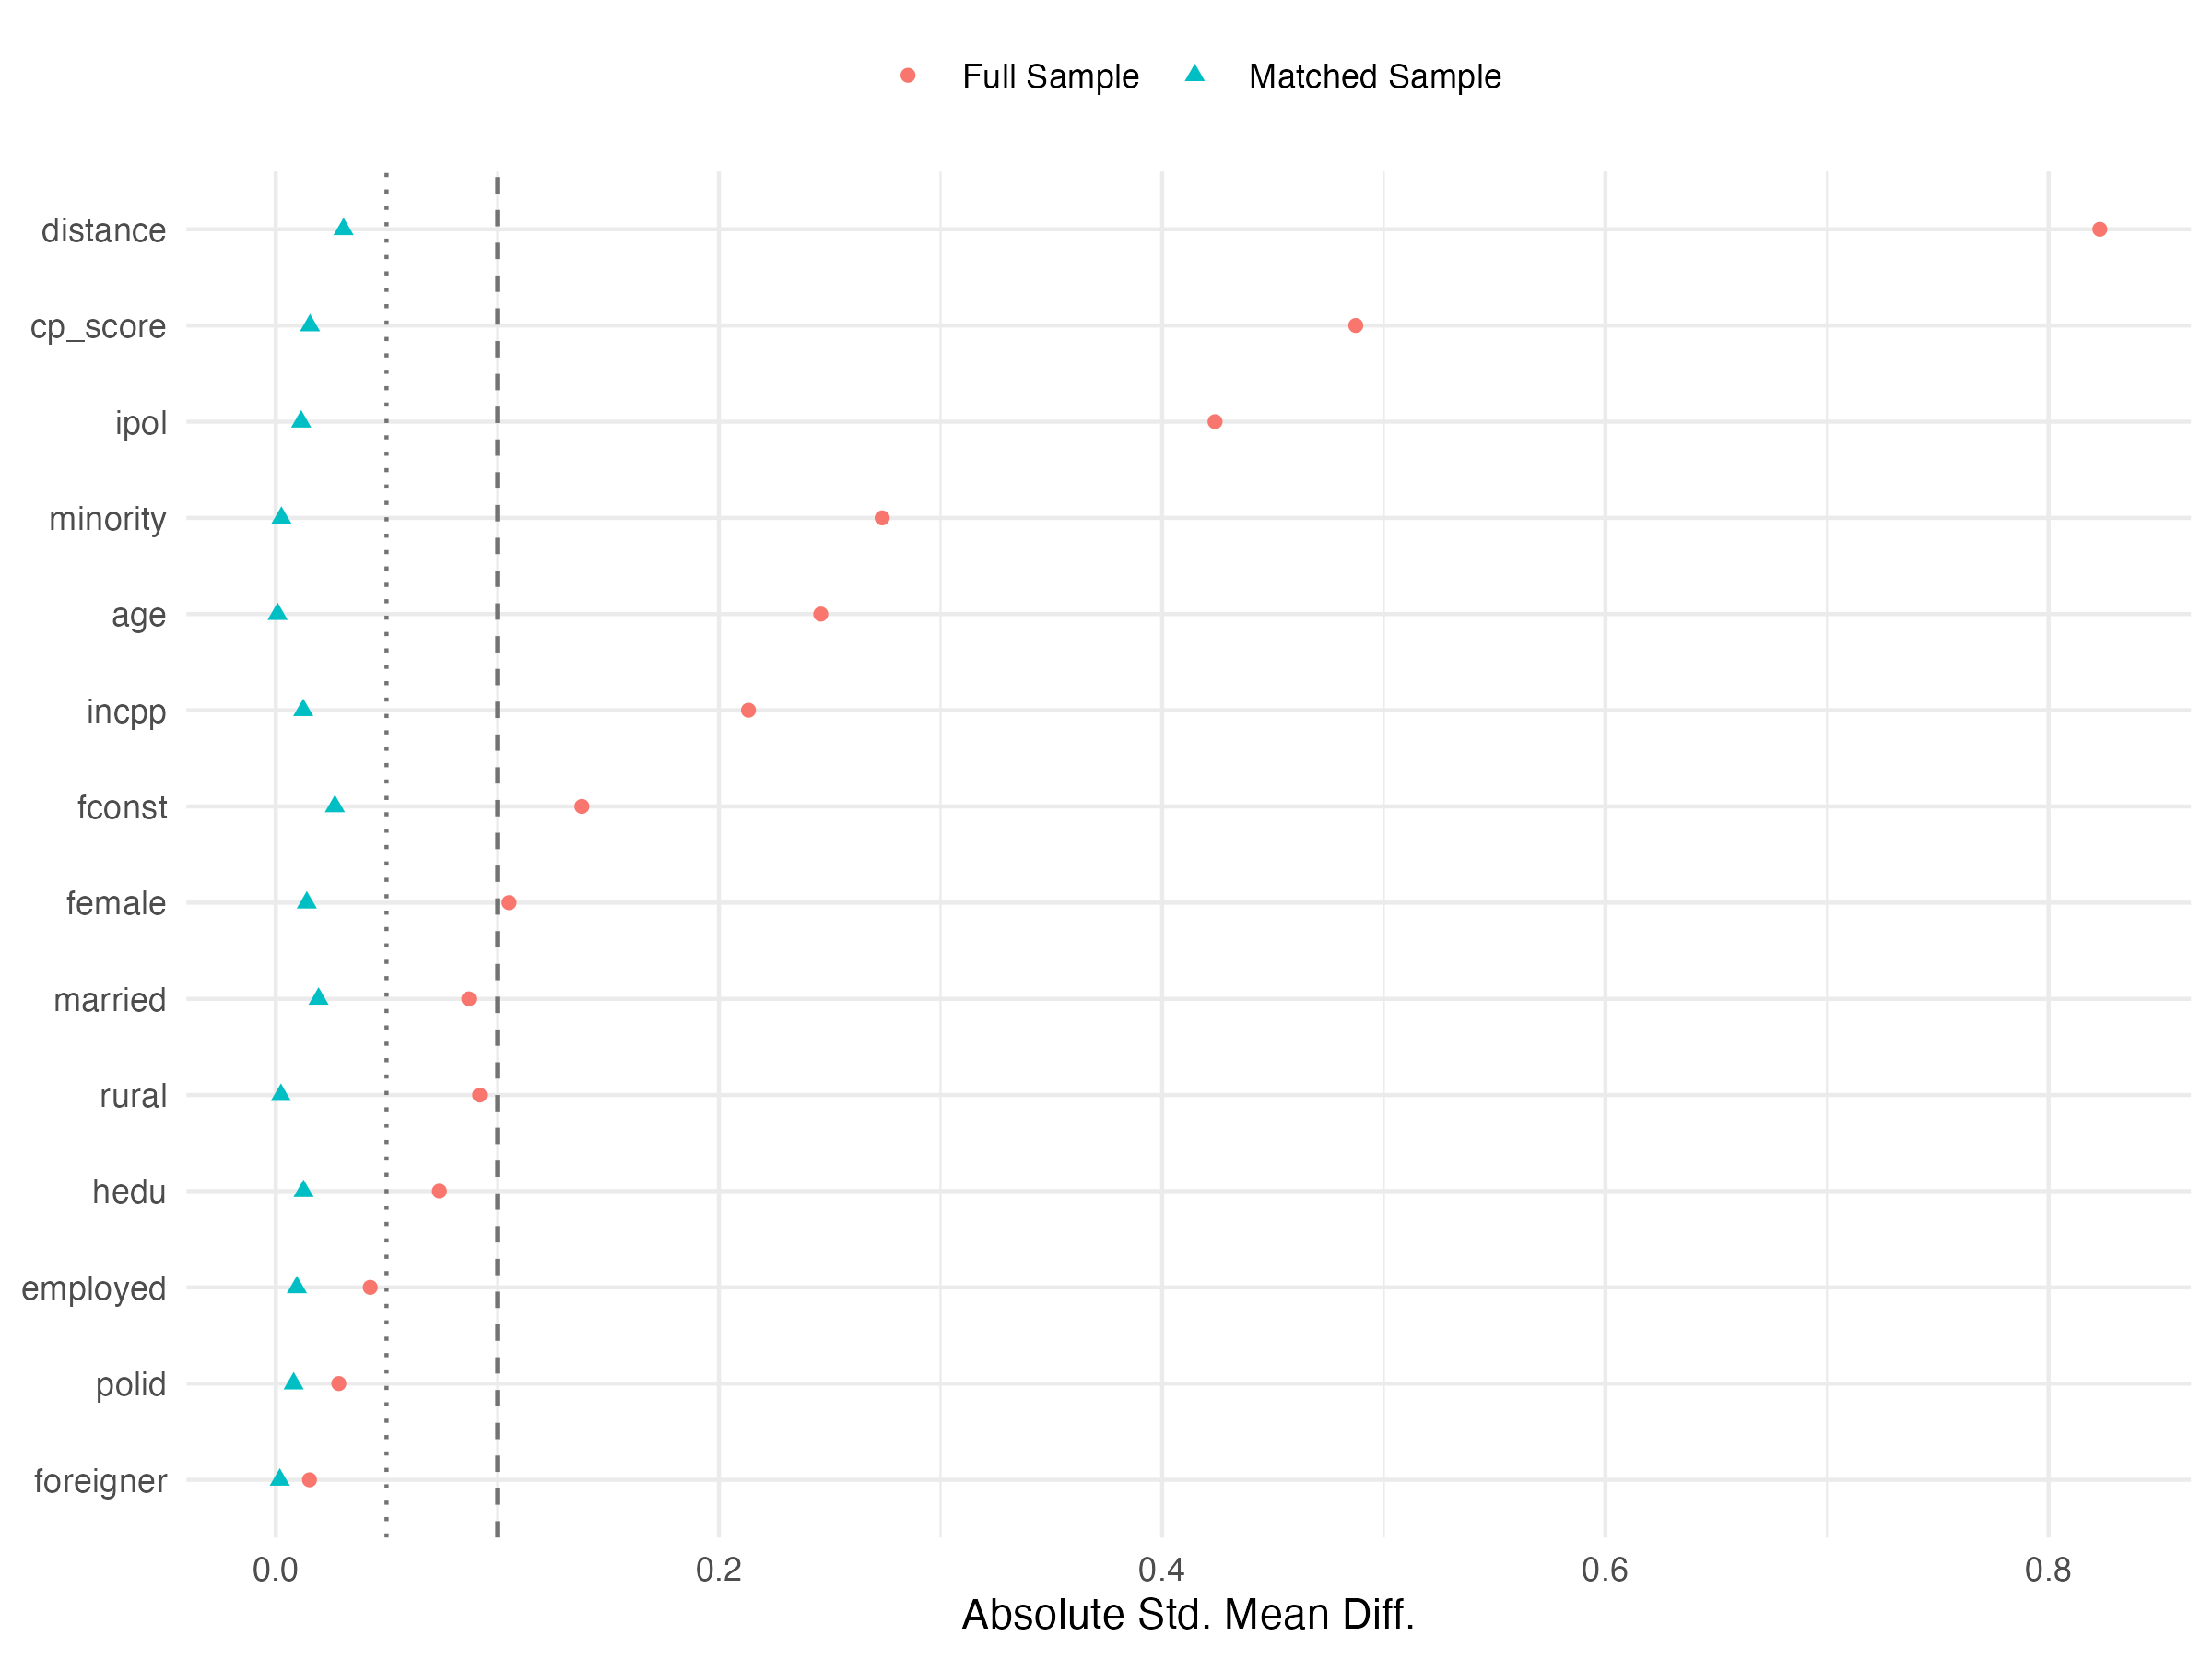
\includegraphics[width=\textwidth]{"viz/loveplot.png"}

\medskip
\justifying\footnotesize 
\textit{Note:} The figure shows the Absolute Std. Mean Diff. for each covariate before (full sample) and after matching. The dashed and dotted lines represent the thresholds of 0.1 and 0.05, respectively, for good balance. The figure indicates that the matching procedure has significantly improved the balance of covariates between the treatment and control groups.

\textit{Source:} Eurovoices General Population Poll 2024
\end{figure}

\newpage
\section{Sensitivity contour plots of point estimates}
\label{appendix:d}
\begin{figure}[htbp]
\centering
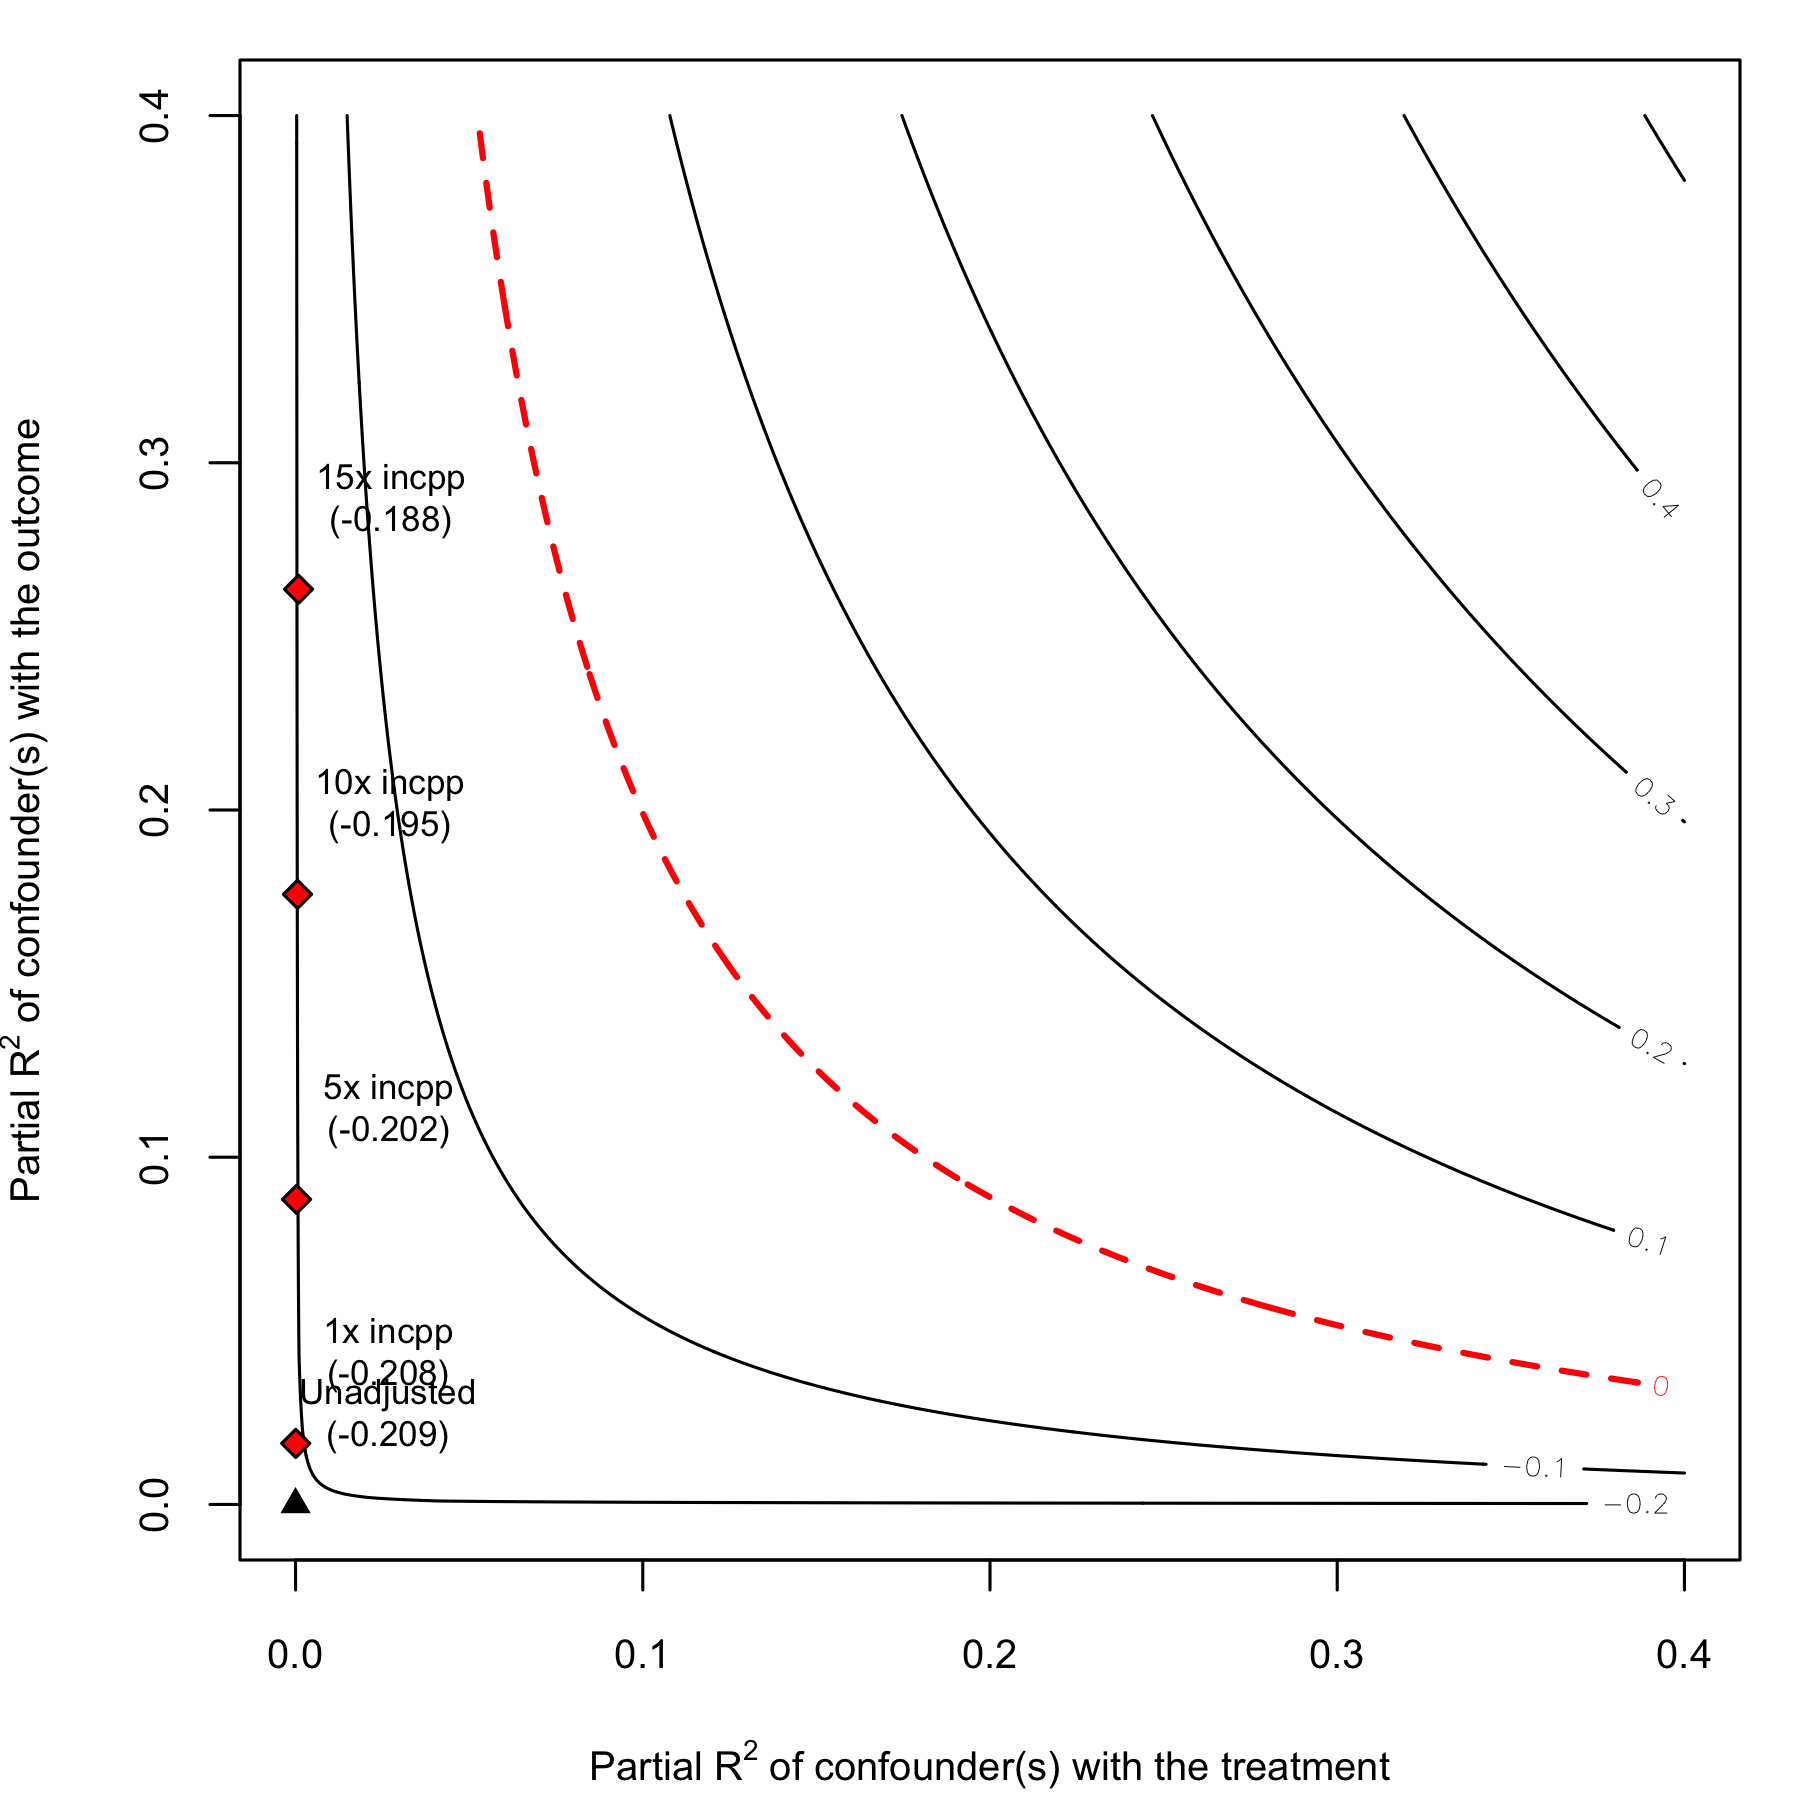
\includegraphics[width=0.95\textwidth]{"viz/sensitivity_analysis.png"}

\medskip
\justifying\footnotesize 
\textit{Note:} The figure shows hypothetical sensitivity contours for the point estimates of the treatment effect of political discrimination and harassment on trust in political institutions. The contours represent the hypothetical residual share of variation of the treatment that an unobserved confounding explains (x-axis) and the the hypothetical partial $R^2$ of an unobserved confounding with the outcome (y-axis). The red line represents the level at which the unobserved confounding would nullify our results. The magnitude of the coefficient of interest (ATT) is shown within parenthesis.

\textit{Source:} Eurovoices General Population Poll 2024
\end{figure}

\end{document}
